
\chapter{Teori}

\begin{draft}

I detta kapitel beskrivs fyra områden av central betydelse för projektet. Dessa områden är domänspecifika språk, begreppen syntax, semantik och syntaxträd, literat progammering samt ARCS-modellen och annan didaktik.

\section{Domänspecifika språk}

Ett domänspecifikt språk är ett språk som är avgränsat till en specifik domän. Nyckelorden är språk, specifik och domän. En domän är ett område, till exempel textformatering eller matlagning. Specifikt syftar på att det är \textit{just detta} område man behandlar och inget mer. Med språk menas ett sätt att uttrycka saker inom domänen. Svenska och Java är två exempel på språk.

Domänspecifika språk används inte bara i programmering utan förekommer även i andra mer vardagliga sammanhang. Inom domänen matlagning är steka, grilla och fritera användbara ord. Likaså inom domänen ridning är grimma, box och galopp användbara ord. Befinner man sig inom domänen vet man vad som menas med grimma och det är ett kort och väldefinerat sätt att uttrycka sig. Men detta språk (här i form av ord och begrepp) är meningslöst utanför domänen. Ett recept kan inte förklaras i termer av grimmor, boxar och galopper.

Domänspecifika språk är vanligt förekommande i programmeringssammanhang. HTML är ett domänspecifikt språk för textformatering, SQL för databashantering och typsnitt för att beskriva hur text ser ut på skärmen. Precis som domänspecifika språk i vardagan passar domänspecifika språk inom programmering enbart sitt egna domän. SQL är bra för databaser men inte att göra ett spel i.

Motsatsen till ett domänspecifikt språk är ett generellt språk. I vardagen är naturliga språk som svenska och engelska generella medan ryttar-begreppen ovan är domänspecifika. Likt i vardagen finns det generella programmeringsspråk som C++ och Java. Dessa är turingkompletta, vilket betyder att det går att uttrycka alla beräkningsbara problem i dem och även lösa dem givet tillräckligt med tid och minnestillgångar.\cite{turing_ne} \cite{turing_book} Begränsningen med dessa generella språk är just deras egen generaliserbarhet, eftersom de har stöd för alla typer av beräkningar så blir både läsbarheten och användarvänligheten lidande.

Ett exempel på ett domänspecifikt språk är \textit{syntaxträd}. Syntaxträd har använts mycket i projektet och beskrivs mer utförligt i avsnitt \ref{sec:syntax}.

Ett domänspecifikt språk kan antingen implementeras som ett fristående språk eller bäddas in i ett redan existerande språk. De domänspecifika språk som utvecklats inom detta projekt är inbäddade i programmeringsspråket \textit{Haskell}. Haskell är ett lämpligt val eftersom det är enkelt att skapa datatyper som bygger upp det domänspecifika språket. Att Haskell är ett högnivå-språk är också en fördel då man slipper programerings-tekniska detaljer, till exempel minneshantering, och istället kan fokusera på programmet innehåll och betydelse. Slutligen gör dess mönstermatchning att de datatyper som utgör det domänspecifika språket enkelt kan brytas isär och manipuleras.

\section{Syntax, semantik och syntaxträd}
\label{sec:syntax}

I samband med domänspecifika språk dyker begreppen \textit{syntax} och \textit{semantik} upp. Syntax är grammatiken för ett språk medan semantiken är betydelsen av en konstruktion, en mening, i språket. Inom aritmetik\footnote{Aritmetik är den gren inom matematiken som behandlar att räkna.} är tal och räknesätt syntax medan uttrycket beräknat är semantiken. Till exempel är $((3 + 2) * 10)^4$ syntax medan $6.250.000$ är semantiken, eftersom det är det som det syntaktiska uttrycket \textit{betyder}. Domänspecifika språk har med syntax att göra eftersom många domänspecifika språk används till att modellera just syntax.

En form av domänspecika språk är syntaxträd, och som redan nämnts har de en stor betydelse i detta projekt. Ett syntaxträd är en trädrepresentation av en syntax. För att illustrera begreppet visas här ett domänspecifikt språk som är ett syntaxträd som modellerar aritmetiska uttryck. Det är implementerat i Haskell. Syntaxträdet visas i figur \ref{fig:syntax_exempel}.

\begin{figure}[tph]
  \begin{lstlisting}
data Expr = Expr :+: Expr
          | Expr :*: Expr
          | Const Double
  \end{lstlisting}
  \caption{Ett syntaxträd i Haskell. Detta är ett exempel på ett litet domänspecifikt språk.}
  \label{fig:syntax_exempel}
\end{figure}

Syntaxträdet innehåller \textit{datakonstruktorer} för att representera \textit{löv} (ändpunkter) och \textit{förgreningar}. I detta exempel är \texttt{:+:} och \texttt{:*:} förgreningar. Med hjälp av dem kan man uttrycka summan respektive produkten av två andra uttryck. Löven representeras av \texttt{Const}, det är en konstant som man ej kan bygga vidare på.

Med datakonstruktorerna kan man konstruera värden i språket. Ett exempelvärde från det tidigare syntaxträdet visas i figur \ref{fig:syntax_exempel_varde}.

\begin{figure}[tph]
  \begin{lstlisting}
value = Const 7 :*: (Const 3 :+: Const 10)
  \end{lstlisting}
  \caption{Ett exempelvärde ur det tidigare syntaxträdet. Detta modellerar det matematiska uttrycket $7 * (3 + 10)$}
  \label{fig:syntax_exempel_varde}
\end{figure}

Figur \ref{fig:syntax_exempel_varde} visar hur det aritmetiska uttrycket $7 * (3 + 10)$ modelleras. Konstruktorn \texttt{:*:} får som sina två argument uttrycken \texttt{Const 7} och \texttt{Const 3 :+: Const 10}. Det är alltså en produkt av två deluttryck. Syntaxträd brukar illusteras med just träddiagram. Detta exempelvärde illustreras i figur \ref{fig:syntax_exempel_bild}.

\begin{figure}[tph]
  \centering
  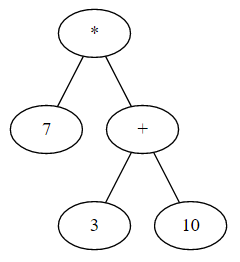
\includegraphics[width=0.4\linewidth]{figure/syntax_exempel_bild.png}
  \caption{Exempelvärde från syntaxträdet illustrerat i ett träddiagram.}
  \label{fig:syntax_exempel_bild}
\end{figure}

Precis som semantik har en roll i samband med syntax, har semantik även en roll i samband med syntaxträd. I detta exempel är semantiken det värde som syntaxträdet betyder. Detta värde kan beräknas utifrån syntaxträdet. Det görs genom en \textit{utvärderingsfunktion}. För exemplets syntaxträd kan utvärderingsfunktionen se ut som i figur \ref{fig:eval_tree}

\begin{figure}[tph]
  \begin{lstlisting}
evaluate :: Expr -> Double
evaluate (e1 :+: e2) = evaluate e1 + evaluate e2
evaluate (e1 :*: e2) = evaluate e1 * evaluate e2
evaluate (Const v)   = v
  \end{lstlisting}
  \caption{En utvärderingsfunktion för syntaxträdet.}
  \label{fig:eval_tree}
\end{figure}

Det finns tre saker speciellt värda att notera i figur \ref{fig:eval_tree}. Det ena är att eftersom syntaxen innehåller tre olika typer av element, här motsvarat av de tre datakonstruktorerna, krävs tre fall i utvärderingsfunktionen som vardera utvärderar ett av dem. \textit{evaluate} har därför ett fall för \texttt{:+:}, ett för \texttt{:*:} och ett för \texttt{Const}. 

Den andra saken att notera ur figur \ref{fig:eval_tree} är hur ett fall utvärderas. Hur utvärderingen ska ses ut får man genom att ta hänsyn till semantiken hos det syntaktiska elementet. \texttt{e1 :+: e2} är syntax för addition av de två uttrycken \texttt{e1} och \texttt{e2}. Därför blir semantiken, värdet, av \texttt{e1 :+: e2} lika med värdet hos \texttt{e1} och \texttt{e2} adderade. Ett liknande resonemang ger svaret på hur utvärderingen av de två resterande fallen ska se ut.

Den tredje saken i figur \ref{fig:eval_tree} värd att poängtera är dess typsignatur, \texttt{Expr -> Double}. Den gör nämligen att man kan tolka \texttt{evaluate}, och utvärderingsfunktioner i allmänhet, som en översättning från syntax (här \texttt{Expr}) till semantik (här \texttt{Double}).

\end{draft}

\section{Litterat programmering och Literate Haskell}
\label{sec:lhs}
\begin{draft}
\textit{Litterat programmering} (engelska \textit{literate programming}) är ett
alternativt sätt att programmera som introducerats av Donald Knuth.\cite{knuth}
Istället för att skriva ett program för en dator, skriver man ett program som
kan läsas både av människor och datorer. Det visar sig på följande två sätt.

Det ena sättet är att jämfört med traditionella program får dokumentationen en
ökad betydelse. I traditionella program är programkoden den viktiga delen. I
litterata program däremot är dokumentationen minst lika viktig. Den används till
att förklara koden, sätta den i relationen till andra delar och så vidare.
Detta jämnbördiga förhållande syns konkret genom att titta på hur källkoden är
skriven i ett literat program. Det kan till exempel se ut som i figur
\ref{fig:litterate_haskell_exempel} där man ser att källkoden och text för
människor är sammanvävda på ett jämnbördigt sätt, där den ena inte är viktigare
än den andra.

\begin{figure}[tph]
  \begin{lstlisting}[language={}]
How does all this tie together? First the type is decided, for instance

> type ExampleType = Quantity T.Length Double

then a value of that type is created

> exampleValue :: ExampleType
> exampleValue = Quantity V.length 5.3

Note that the Quantity data type has both value-level and type-level dimensions. As previosuly mentioned, value-level in order to print prettily and type-level to only permit legal operations.
  \end{lstlisting}
  \caption{Ett exempel på hur en källfil till litterat programmering kan se ut. Exemplet är Litterate Haskell. Rader som börjar med \texttt{>} markerar att det är progamkod, medan rader utan markerar att det är text för människor.}
  \label{fig:litterate_haskell_exempel}
\end{figure}

Det andra sättet ett litterat program skiljer sig åt är ordningen programkoden
står i. Traditionell programmering börjar oftast med att definiera små funktioner
och metoder med snäva användningsområden och använder sen dessa för att senare
bygga ihop mer komplexa strukturer. Med literat programmering börjar man hellre
med den komplexa strukturer först och skriver text som förklarar den generella
struktureren utan att gå in på detaljerna, för att sedan presentera de små
delarna var för sig med tillhörande förklarande text.

\textit{Litterate Haskell} är literat programmering för Haskell.\cite{litterate_haskell}
Att programmera i Litterate Haskell går till på samma sätt som vanlig Haskell,
med skillndaden att programkod och text vävs ihop i en och samma fil. Det kan
se ut som i figur \ref{fig:litterate_haskell_exempel}. Filen, med tillägget
\texttt{.lhs}, går att använda direkt med Haskell-kompilatorn GHC. All text
ignoreras och programkoden behandlas som om den var en vanlig
Haskell-fil. \texttt{.lhs}-filen kan också kompileras till material avsett för
mäniskor. Det finns flera verktyg som gör det men det som används i detta
projekt är \textit{Pandoc}\cite{pandoc}. Med \textit{Pandoc} kan texten märkas
up med både \texttt{markdown} (används i projektet) och \texttt{Latex}. Det går
att exportera till bland annat HTML och PDF.
\end{draft}

\section{Att skapa motiverande läromaterial}
\label{sec:arcs}
\begin{binge}
ARCS-SAKER

Motivation är en persons vilja att göra något. I undervisningssammanhang vill man att studenten ska lära sig materialet. Studenten behöver alltså vara motiverad, att vilja, lära sig. Motivation kan ha flera källor. Till exempel att studenten tycker materialet är intressant eller att det finns belöningar i form av tillfredsställelsen att få att högt betyg. 

\textit{Motiverande design} innebär att systematiskt utforma undervisningen på ett sådant sätt att studenten blir motiverad till att lära sig. Det handlar om att använda olika tekniker för att väcka och behålla motivation. Det finns ett flertal olika modeller för detta men i detta projekt används enbart den så kallade \textit{ARCS}-modellen.\cite{arcs_book}

\textit{ARCS} är en förkortning av ''Attention, Relevance, Confidence and Satisfaction'', på svenska ''uppmärksamhet, relevans, självförtroende och tillfredsställelse''. Precis som namnet antyder innehåller modellen fyra delar som vardera behandlar en aspekt av motivation. \textit{Attention} handlar om att fånga uppmärksamhet och väcka nyfikenhet. \textit{Relevance} handlar om att tillgodose studentens behov så att materialet upplevs som relevant för hen. \textit{Confidence} handlar om att övertyga studenten att hen kommer kunna lyckas lära sig materialet. \textit{Satisfaction} handlar om att ge studenten tillfredställelse efter att ha lärt sig något så att hen vill fortsätta lära sig. Det finns strategier för hur man genomför de olika delarna i praktiken och här följer en översikt för \textit{Attention}.\footnote{Eftersom projektet har ett begränsat fokus på de pedagogiska aspekterna, se avsnitt \ref{sec:avgransningar}, har enbart \textit{Attention} och \textit{Confidence} tagits hänsyn till. Av det skälet är det enbart de två delarna beskrivna här.}

För att fånga studentens uppmärksamhet och intresse finns tre allmäna strategier. Den första är varselblivning, att något plötsligt händer som man blir medveten om. Det kan till exempel åstadkommas genom överraskande information, en förändring i ljuset i en föreläsning eller att humor vävs in. Den andra är att väcka nyfikenhet. Ett par sätt för det är att involvera mystik i miljön och att ställa frågor. Det tredje sättet är variation. Då handlar det om olika struktur och ordning på utlärningen, till exempel att inte alltid utforma en lektion som föreläsning, demonstration och sedan övning, utan variera det med andra inslag, exempelvis ett filmklipp.

BJÖRN-SAKER

Lärande Skola Bildning - kap 5 lärandeteorier

Knyta an materialets undervisningspotential till lärandeteorier.

Vygotskij - Sociokulturella lärandet (ex parprogrammering + diskussion emellan individer)

Jean Piaget - Kognitivismen (lära sig A, B, A + B -> C, alternativt att eleven utmanas med något den trodde var sant, och tvingas omformulera en lösning som stödjer den presenterade situationen).

Skinner - Behaviorism (ex glada tomater vs wall of text? Det är väll egentligen detta som hindrar läsare att läsa en "tråkig, tung svårläst text")
Vi väver in det som elever inte förknippar med tunga texter -> färre flyktförsök.

\iffalse
Skulle vilja hitta stöd för:
Bara något som olika bakgrunder skulle kunna ge en inbillning av miljöombyte, vilket minskar den monotona dimensionen, och i sig förhindrar hjärnans anti-"get-stuck-on-a-thought-and-die".
\fi

\end{binge}
